\chapter{Návrh a~implementace identifikace s~využitím JA3/JA4 otisků a~frekventovaných vzorů}
\label{chp:design}
Tato kapitola se zaměřuje na~návrh a~implementaci systému pro~identifikaci síťových aplikací s~využitím otisků \textit{JA3} a~\textit{JA4} v~kombinaci s~analýzou frekventovaných vzorů. Nejprve jsou představeny použité datové sady, jejich původ, struktura a~proces předzpracování. Následně je podrobně popsán návrh systému, jeho architektura a~zvolené metody pro~extrakci charakteristických rysů síťové komunikace. Důraz je kladen na~praktickou implementaci řešení, včetně využití algoritmů pro~dolování častých vzorů a~zpracování otisků v~prostředí jazyka \textit{Python}. Cílem této kapitoly je nejen popsat samotný postup realizace systému, ale také zdůvodnit výběr konkrétních technologií a~metod, které byly v~rámci vývoje zvoleny.

\section{Seznámení s~datovými sadami}
\label{sec:dataset}
Pro účely této práce byly poskytnuty tři datové sady: \texttt{mobile\_desktop\_apps\_raw.csv} (autor -- Fakulta informačních technologií, Vysoké učení technické v~Brně ), \texttt{iscx.csv} a~\texttt{iscx-raw.csv} (autor -- Univeristy of New Brunswick, Canadian Institute for Cybersecurity). Tyto soubory obsahují záznamy o~šifrované síťové komunikaci navázané pomocí protokolu \textit{TLS}, konkrétně o~jednotlivých spojeních generovaných různými aplikacemi v~kontrolovaném testovacím prostředí. Každý řádek reprezentuje jedno \textit{TLS} spojení a~popisuje informace získané jak z~klientské zprávy \texttt{Client Hello}, tak ze zprávy \texttt{Server Hello}, které se vyměňují při~navazování šifrovaného spojení.

Datové sady byly využity v~předchozích výzkumech zaměřených na~analýzu šifrovaného provozu a~identifikaci síťových aplikací~\cite{MatousekMobileDevice2020}~\cite{BurgetovaJA42024}. 

Následuje popis jednotlivých souborů:

\begin{itemize}
	\item \textbf{iscx.csv} -- Základní verze datové sady, která obsahuje agregované informace o~spojeních. Klíčové sloupce zahrnují:
	      \begin{itemize}
	      	\item \texttt{SrcIP}, \texttt{DstIP}, \texttt{SrcPort}, \texttt{DstPort} -- informace o~zdrojové a~cílové \textit{IP} adrese a~portech,
	      	\item \texttt{SNI} -- \textit{Server Name Indication}, doménové jméno cílového serveru,
	      	\item \texttt{OrgName}\footnote{OrgName – Organizace odpovídající \textit{IP} adresy serveru, získané z~databáze \textit{WHOIS}.} -- organizace provozující cílový server (např. Google, Skype),
	      	\item \texttt{JA3hash}, \texttt{JA4hash} -- otisky \textit{TLS} klienta dle metod \textit{JA3} a~\textit{JA4},
	      	\item \texttt{JA3Shash}, \texttt{JA4Shash} -- otisky \textit{TLS} serveru dle metod \textit{JA3S} a~\textit{JA4S},
	      	\item \texttt{AppName}\footnote{Nejedná se o~přesné názvy aplikací ale pouze o~jejich zkratky.} -- zkratka názvu aplikace generující provoz (např. Skype, Hangouts),
	      	\item \texttt{Type} -- typ provozu: \texttt{0} (běžná aplikace), \texttt{M} (škodlivý software), \texttt{A} (reklamní či analytický provoz),
	      	\item \texttt{Filename}\footnote{Reprezentuje název souboru, ze kterého byla datová sada poskládána. V~rámci jednoho souboru je zaznamenáno několik spuštění vždy jedné aplikace.} -- název původního souboru, ze kterého byl záznam extrahován,
	      	\item \texttt{Version} -- verze aplikace, (nepoužívaná, vždy \texttt{0}).
	      \end{itemize}
	      	      	      	      	      
	\item \textbf{iscx-raw.csv} -- Rozšířená verze předešlé sady, obsahující detailní \textit{TLS} metadata včetně obsahu jednotlivých \textit{TLS} parametrů:
	      \begin{itemize}
	      	\item \texttt{Proto} -- typ transportního protokolu (např. TCP = \texttt{6}),
	      	\item \texttt{TLSVersion}, \texttt{ClientCipherSuite}, \texttt{ClientExtensions}, \texttt{SignatureAlgorithms}, \texttt{ClientSupportedGroups} -- detailní \textit{TLS} parametry zaslané klientem,
	      	\item \texttt{ServerCipherSuite}, \texttt{ServerExtensions}, \texttt{ServerSupportedVersions} -- odpovídající parametry na~straně serveru,
	      	\item \texttt{JA4\_raw}, \texttt{JA4S\_raw} -- surové podoby otisků.
	      \end{itemize}
	      	      	      	      	      
	\item \textbf{mobile\_desktop\_apps\_raw.csv} -- Podobná struktura jako \texttt{iscx-raw.csv}, avšak data pochází z~oddělené studie zaměřené na~mobilní a~desktopové aplikace~\cite{MatousekMobileDevice2020}. 
	      Přítomny jsou také sloupce jako:
	      \begin{itemize}
	      	\item \texttt{ALPN} -- protokoly vyjednané při~\textit{TLS handshake} (např. \texttt{http/1.1}, \texttt{h2}),
	      	\item \texttt{ClientSupportedVersions} -- seznam verzí \textit{TLS} podporovaných klientem,
	      \end{itemize}
\end{itemize}
Tabulka~\ref{tab:iscx} níže uvádí statistické charakteristiky vybraných atributů obsažených v~datové sadě \texttt{iscx.csv}\footnote{Kromě atributu \texttt{ClientExtensions} jsou všechny uvedené atributy pouze z~datové sady \texttt{iscx.csv}, neboť \texttt{iscx-raw.csv} ji pouze rozšiřuje o~dodatečná metadata.}. Pro~každý atribut je uveden počet unikátních hodnot, podíl unikátních hodnot vůči celkovému počtu záznamů (v\,\%), celkový počet výskytů atributu, podíl výskytů vzhledem k~celkovému počtu řádků v~datové sadě (v\,\%). Tato statistika slouží k~posouzení informační hodnoty jednotlivých atributů pro~účely identifikace.
\begin{table}[H]
	\centering
	\begin{tabular}{lrlrl}
		\toprule
		\textbf{Položky} & \textbf{Počet unikátních hodnot} & \textbf{( v\,\%)} & \textbf{Celkový počet} & \textbf{( v\,\%)} \\
		\midrule
		SNI               & 207                                 & 8{,}50            & 2092                     & 85{,}88           \\
		OrgName           & 72                                  & 2{,}96            & 2300                     & 94{,}42           \\
		ClientExtensions  & 32                                  & 1.31              & 2436                     & 100.00            \\
		JA3hash           & 46                                  & 1{,}89            & 2436                     & 100{,}00          \\
		JA4hash           & 42                                  & 1{,}72            & 2436                     & 100{,}00          \\
		AppName           & 16                                  & 0{,}66            & 2436                     & 100{,}00          \\
		JA3Shash          & 117                                 & 4{,}80            & 2399                     & 98{,}48           \\
		JA4Shash          & 127                                 & 5{,}21            & 2399                     & 98{,}48           \\
		Filename          & 109                                 & 4{,}47            & 2399                     & 98{,}48           \\
		Type              & 2                                   & 0.08              & 2436                     & 100.00            \\
		\bottomrule
	\end{tabular}
	\caption{Přehled položek v~datové sadě \texttt{iscx.csv}}
	\label{tab:iscx}
\end{table}

Tabulka~\ref{tab:mobile} rozšiřuje statistickou analýzu na~datovou sadu \texttt{mobile\_desktop\_apps\_raw}. Opět jsou uvedeny klíčové atributy relevantní pro~identifikaci aplikací.

\begin{table}[H]
	\centering
	\begin{tabular}{lrlrl}
		\toprule
		\textbf{Položky} & \textbf{Počet unikátních hodnot} & \textbf{( v\,\%)} & \textbf{Celkový počet} & ( \textbf{v\,\%)} \\
		\midrule
		SNI               & 929                                 & 4.36              & 21259                    & 99.80             \\
		OrgName           & 197                                 & 0.92              & 21273                    & 99.87             \\
		ClientExtensions  & 10462                               & 49.12             & 21301                    & 100.00            \\
		ALPN              & 9                                   & 0.04              & 19505                    & 91.57             \\
		JA3hash           & 10495                               & 49.27             & 21301                    & 100.00            \\
		JA4hash           & 123                                 & 0.58              & 21301                    & 100.00            \\
		AppName           & 78                                  & 0.37              & 21301                    & 100.00            \\
		JA3Shash          & 83                                  & 0.39              & 21180                    & 99.43             \\
		JA4Shash          & 103                                 & 0.48              & 21180                    & 99.43             \\
		Filename          & 1746                                & 8.20              & 21180                    & 99.43             \\
		Version           & 1                                   & 0.00              & 21180                    & 99.43             \\
		\bottomrule
	\end{tabular}
	\caption{Přehled položek v~datové sadě \texttt{mobile\_desktop\_apps\_raw.csv}}
	\label{tab:mobile}
\end{table}

V prvních dvou datových sadách, \texttt{iscx.csv} a~\texttt{iscx-raw.csv}, se nachází \textbf{celkem 2436 záznamů}, které byly vygenerovány \textbf{16 různými aplikacemi}. Tyto záznamy pocházejí ze \textbf{109 různých spuštění} (atribut \textit{Filename}). Otisky \textit{JA3} a~\textit{JA4} jsou dostupné pro~každý záznam, zatímco otisky \textit{JA3S} a~\textit{JA4S} chybí přibližně u~1,52\,\% záznamů.

Lze si rovněž povšimnout, že atribut \textit{SNI}, ačkoliv chybí u~14,12\,\% záznamů, obsahuje \textbf{největší počet unikátních hodnot}. Díky tomu se jeví jako ideální kandidát pro~přesnější identifikaci aplikací -- zejména v~případech, kdy dochází ke~zlepšení identifikace kombinací více atributů.

Datová sada \texttt{mobile\_desktop\_apps\_raw.csv} obsahuje \textbf{celkem 21301 záznamů}, které byly vygenerovány \textbf{78 různými aplikacemi}. Dále zahrnuje \textbf{1746 odlišných spuštění} (atribut \texttt{Filename}). Stejně jako u~předchozích datových sad nechybí žádný z~otisků \textit{JA3} ani \textit{JA4}. Naopak otisky \textit{JA3S} a~\textit{JA4S} chybí ve~0,57\,\% případů.

Zajímavý je poměr počtu otisků \textit{JA3} ku~\textit{JA4}, který činí přibližně \textbf{85:1} (10495 ku~123). Tento výrazný nepoměr naznačuje, že informační hodnota otisků \textit{JA3} může být silně ovlivněna přímo použitými rozšířeními (např. \texttt{ClientExtensions}), kterých je v~datasetu evidováno 10462, viz~\ref{sec:JA3}. Na~rozdíl od~\textit{JA4}, jehož konstrukce počítá s~filtrováním redundancí pomoci seřazení a~výpočtu zkráceného hashe, se \textit{JA3} otisk generuje ze všech rozšíření bez~jakýchkoli úprav, což může vést ke~snížení jeho spolehlivosti pro~účely identifikace.

Opět i~v~tomto případě se položka \textit{SNI} jeví jako \textbf{vhodný kandidát pro~přesnější identifikaci}, neboť vykazuje vysoký počet unikátních hodnot a~chybí pouze ve~0,2\,\% záznamů, což svědčí o~její vysoké informační hodnotě.

Tabulky~\ref{tab:apps-iscx} a~\ref{tab:apps-mobile} poskytují přehled o~rozložení aplikací v~jednotlivých použitých datových sadách. Každá tabulka uvádí název aplikace, počet zaznamenaných spojení a~relativní podíl na~celkovém počtu spojení v~dané datové sadě.
Tabulka~\ref{tab:apps-iscx} shrnuje statistiky z~datové sady \texttt{iscx.csv}, kde dominují zejména aplikace jako \textit{Hangouts} a~\textit{Skype}.
Taktéž tabulka~\ref{tab:apps-mobile} zachycuje rozložení aplikací v~rozsáhlejší datové sadě \texttt{mobile\_desktop\_apps\_raw.csv}, která obsahuje širší spektrum moderních mobilních i~desktopových aplikací.

Pro přehlednost jsou v~obou tabulkách uvedeny pouze vybrané položky -- prostřední části byly nahrazeny výpustkami.

\begin{table}[H]
	\centering
	\begin{minipage}{0.49\textwidth}
		\centering
		\begin{tabular}{lll}
			\toprule
			\multicolumn{3}{c}{\texttt{iscx.csv}} \\
			\midrule
			\textbf{Aplikace} & \textbf{Počet} & \textbf{Podíl (\%)} \\
			\midrule
			Hangouts          & 553             & 22.70                \\
			Skype             & 436             & 17.90                \\
			Email             & 315             & 12.93                \\
			\vdots            & \vdots          & \vdots               \\
			SCP               & 9               & 0.37                 \\
			BitTorrent        & 8               & 0.33                 \\
			ICQ               & 7               & 0.29                 \\
			\bottomrule
		\end{tabular}
		\caption{Přehled aplikací v~\texttt{iscx.csv}}
		\label{tab:apps-iscx}
	\end{minipage}
	\hfill
	\begin{minipage}{0.49\textwidth}
		\centering
		\begin{tabular}{lll}
			\toprule
			\multicolumn{3}{c}{\texttt{mobile\_desktop\_apps\_raw.csv}} \\
			\midrule
			\textbf{Aplikace} & \textbf{Počet} & \textbf{Podíl (\%)} \\
			\midrule
			AirDroid          & 1774            & 8.33                 \\
			Oer               & 1441            & 6.76                 \\
			BiduTerBox        & 1252            & 5.88                 \\
			\vdots            & \vdots          & \vdots               \\
			Milbird           & 15              & 0.07                 \\
			Telegram          & 12              & 0.06                 \\
			TelegramDesktop   & 1               & 0.01                 \\
			\bottomrule
		\end{tabular}
		\caption{Přehled aplikací v~3. sadě}
		\label{tab:apps-mobile}
	\end{minipage}
\end{table}


Všechny tři datové sady se všemi atributy, včetně kompletního seznamu aplikací použitých v~těchto sadách, jsou uvedeny v~příloze~\ref{chp:appendix-ds}.


\section{Motivace a~obecný popis}
Tato sekce poskytuje obecný přehled o~navrženém řešení, jeho struktuře a~zvoleném přístupu. Hlavním cílem této práce je zlepšit identifikaci aplikací prostřednictvím kontextového přístupu. Při~aplikaci otisku na~identifikované spojení je vygenerována kandidátní množina aplikací, tedy množina všech aplikací, ke~kterým je daný otisk přiřazen v~trénovací fázi. Tato kandidátní množina je tedy výsledkem metod, jako jsou \textit{JA3} nebo \textit{JA4}, pokud jsou použity k~identifikaci \textit{TLS} spojení. Identifikace založená výhradně na~otiscích, přestože může na~první pohled působit poměrně přesně, není ideální – průměrná velikost kandidátní množiny bývá často příliš rozsáhlá, což snižuje její informační hodnotu.

Například v~situaci, kdy 16 odlišných aplikací generuje síťovou komunikaci, může klasifikace založená na~otiscích vrátit kandidátní množinu o~velikosti 14. Takový výsledek je z~hlediska jednoznačné identifikace aplikace prakticky bezcenný, protože neposkytuje dostatečně úzký výběr možných odpovědí. 

Cílem této práce je pokusit se zúžit kandidátní množinu tak, aby bylo možné dosáhnout přesnější identifikace aplikace, a~to na~základě kontextu dalších \textit{TLS} spojení, která se vyskytují paralelně s~daným spojením. Využití kontextu dalších \textit{TLS} spojení je možné díky tomu, že většina aplikací při~spuštění generuje více souběžných spojení~\cite{tls-mulitple-conns}. V~rámci těchto okolních \textit{TLS} spojení se hledají frekventované vzory, založené na~otiscích a~případně i~dalších atributech komunikace. Na~základě shody mezi~aktuálním okolím spojení a~předem známými frekventovanými vzory je následně možné určit nejpravděpodobnější kandidáty pro~identifikaci aplikace. 

\section{Návrh řešení}
Tato kapitola se věnuje detailnímu návrhu systému. Na~základě analýzy současných metod a~problémů spojených s~identifikací na~základě otisků je zde představen nový přístup, který využívá informace o~souběžně navázaných \textit{TLS} spojeních.

Cílem návrhu je vytvořit systém, který dokáže efektivně využít kontextové informace k~zúžení kandidátní množiny aplikací, a~tím zlepšit přesnost výsledné identifikace. Sekce popisuje požadavky na~systém, jeho architekturu, zvolené algoritmy a~metodiky, předpoklady pro~jeho fungování i~jednotlivé klíčové části řešení.


\subsection{Požadavky a~cíle}

Jak již bylo zmíněno, hlavním cílem této práce je především zúžení kandidátní množiny pomocí kontextového přístupu. Zároveň je žádoucí, aby byla zachována co nejvyšší přesnost identifikace a~aby zpracování spojení nebylo časově náročné. Je proto nutné nalézt ideální kompromis mezi~přesností a~časovou náročností, což samo o~sobě může být náročné.

\subsection{Architektura systému}
\label{sub:architecture}
Z~důvodu rozšiřitelnosti a~snadnější manipulace byl zvolen přístup objektově orientovaného programování. Systém je rozdělen do~několika vzájemně spolupracujících tříd, které odpovídají jednotlivým částem řešení – načítání a~uchovávání dat, identifikace založená čistě na~otiscích, učení frekventovaných vzorů a~kombinace identifikace otisků s~kontextovým přístupem. Součástí systému jsou i~třídy pro~logování, správu nastavení a~parsování parametrů z~příkazové řádky. Tento přístup zajišťuje lepší modularitu, snadnější rozšiřování funkcionality a~přehlednou správu celkového kódu. Diagram tříd~\ref{fig:class-dia} poskytuje podrobný přehled jednotlivých tříd a~jejich metod.

\begin{figure}[H]
	\centering
	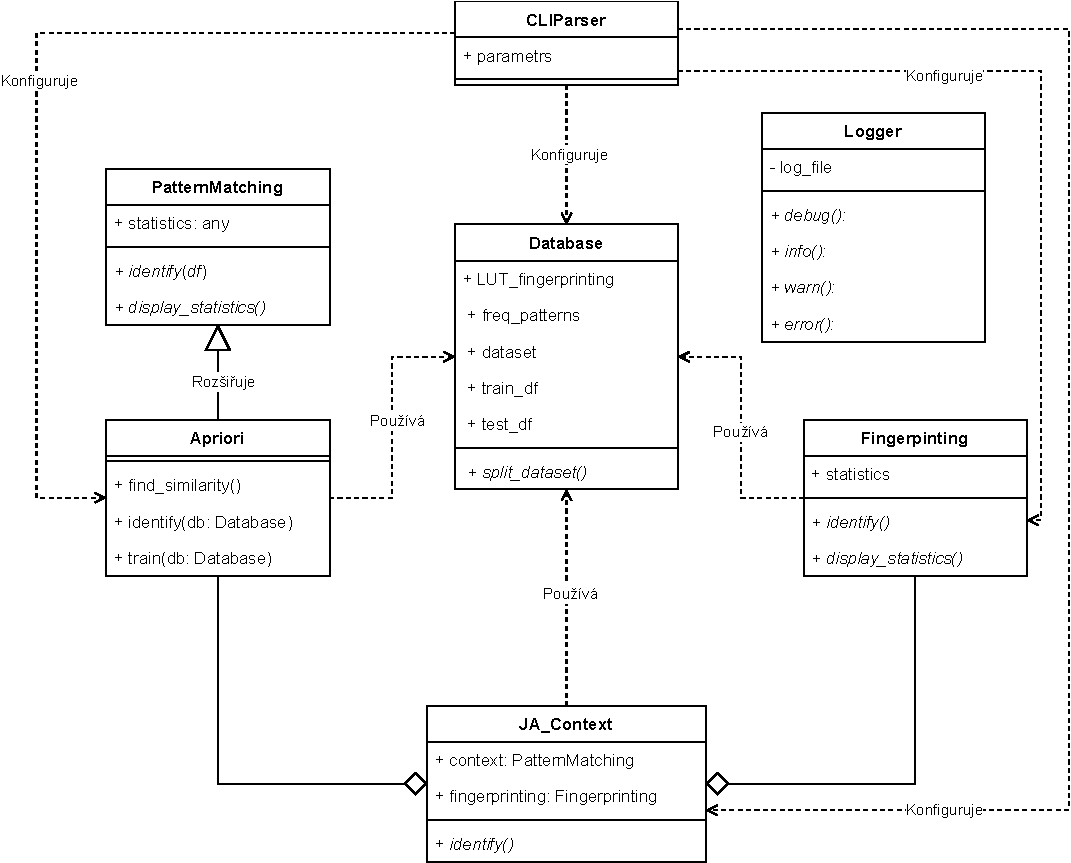
\includegraphics[width=\textwidth]{obrazky-figures/class-dia.drawio.pdf}
	\caption{Diagram tříd}
	\label{fig:class-dia}
\end{figure}


V příloze~\ref{chp:appendix-class-diagram} je uvedena rozšířená verze diagramu tříd, která obsahuje všechny atributy a~metody.

Navržené řešení se bude skládat ze sedmi tříd, přičemž každá z~nich pokryje jasně vymezenou část systému. Ovládání systému bude zajištěno prostřednictvím příkazové řádky, což vyžaduje existenci třídy \texttt{CLIParser}, která zpracuje parametry programu a~předá je příslušným instancím ostatních tříd, jak je znázorněno v~diagramu~\ref{fig:class-dia}.

Pro účely snadného ladění a~lepšího porozumění běhu programu se každý významný krok bude zaznamenávat prostřednictvím instance třídy \texttt{Logger}.

Třída \texttt{Database} bude sloužit jako hlavní zdroj dat a~poskytne přístup k~vyhledávací tabulce otisků, datové struktuře frekventovaných vzorů a~dalším potřebným údajům z~trénovací i~testovací části datové sady. Přístup k~těmto datům bude mít každá komponenta, která je bude vyžadovat.

Třída \texttt{Fingerprinting} nabídne metody pro~identifikaci \textit{TLS} spojení pomocí otisků \textit{JA3}, \textit{JA4} či jejich kombinací (\textit{JA} + \textit{JAS} + \textit{SNI}), přičemž bude využívat vyhledávací tabulku uloženou v~databázi. Zároveň bude zajišťovat generování statistik, které zaznamenají například přesnost identifikace nebo velikost kandidátní množiny.

Třída \texttt{PatternMatching} vytvoří základní rozhraní pro~implementaci algoritmů určených k~dolování informací z~dat. Její návrh umožní snadné rozšíření systému o~další metody data miningu a~zajistí tak jeho flexibilitu a~rozšiřitelnost.

Třída \texttt{Apriori} rozšíří třídu \texttt{PatternMatching} o~konkrétní implementaci algoritmu \textit{Apriori}. Tento algoritmus umožní vyhledávání frekventovaných vzorců v~trénovacích datech a~bude spolupracovat s~databází pro~jejich ukládání a~vyhledávání. Porovnávat nalezené vzory se zkoumaným \textit{TLS} spojením a~vracet N\footnote{Kde N~reprezentuje předem určený maximální počet kandidátů.} nejpravděpodobnějších kandidátů na~základě podobnosti, vypočítané například porovnáním otisků nebo frekvence vzorců, bude metoda \texttt{find\_similarity()}.

Třída \texttt{JA\_Context} bude koordinovat využití tříd \texttt{Apriori} a~\texttt{Fingerprinting} s~cílem zúžit kandidátní množinu pro~identifikaci aplikace. Nejprve provede iteraci přes testovací data v~rámci předem definovaného okna a~tím specifikuje okolí analyzovaného spojení. Pomocí otisků vytvoří počáteční kandidátní množinu aplikací, které budou relevantní pro~dané spojení. Následně předá odpovídající frekventované vzory těchto kandidátů instanci třídy \texttt{Apriori}, která se pokusí nalézt vzory charakteristické pro~aplikace v~dané oblasti. Výsledkem tohoto procesu bude dále zúžená kandidátní množina obsahující aplikace nejlépe odpovídající analyzovanému spojení.

\subsection{Předpoklady a~omezení}
Pro správné spuštění a~fungování systému je nutné splnit několik základních předpokladů:
\begin{itemize}
	\item \textbf{Dostupnost datové sady}: Program vyžaduje existenci pojmenované datové sady obsahující alespoň čtyři TLS spojení, přičemž každé musí obsahovat otisky \textit{JA3} a~\textit{JA3S} (případně \textit{JA4} a~\textit{JA4S}) a~atribut \textit{SNI}. Bez~datové sady nebude možné program spustit.
	\item \textbf{Kvalita a~rozsah dat}: Platí, že čím více unikátních spuštění aplikací je v~datové sadě zaznamenáno, tím rozsáhlejší a~přesnější frekventované vzory je možné extrahovat. Malé množství dat povede ke~snížení přesnosti identifikace. Ovšem také velmi rozsáhlé datové sady mohou zvýšit nároky na~paměť a~výpočetní výkon. Návrh systému je optimalizován pro~běžné datové sady (například \texttt{mobile\_desktop\_apps\_raw.csv}, která obsahuje 21,301 řádků, je v~tomto případě považována za~běžnou datovou sadu).
\end{itemize}

\section{Implementace}
Tato sekce popisuje implementační detaily, použité technologie a~poskytuje podrobný popis klíčových částí systému.

\subsection{Použité technologie a~nástroje}
Pro implementaci byl zvolen programovací jazyk \textit{Python} verze 3.13 kvůli vysoké flexibilitě a~dostupnosti knihoven jak pro~práci s~daty, tak pro~matematické výpočty a~další účely. \textit{Python} také usnadňuje implementaci objektově orientovaného návrhu.

Za účelem efektivní práce s~datovou sadou byla zvolena knihovna \textit{Pandas} verze 2.2.3. Algoritmus \textit{Apriori} byl importován z~knihovny \textit{mlxtend} verze 0.23.4, stejně jako \textit{TransactionEncoder}, který je potřebný pro~předzpracování dat. Knihovna \textit{scikit\_learn} verze 1.6.1 poskytla metodu \texttt{train\_test\_split} pro~rozdělení datové sady na~testovací a~trénovací část, a~také metodu \texttt{cosine\_similarity} pro~výpočet kosinové podobnosti. Knihovna \textit{numpy} verze 2.2.5 byla také využita pro~různé matematické operace. Při tvorbě této technické zprávy byla využita umělá inteligence, konkrétně \textit{ChatGPT}, pro úpravu stylistiky a opravu gramatiky.


\subsection{Použití programu a~konfigurace}
K zajištění správného běhu programu a~korektního zpracování dat byl vytvořen konfigurační soubor \texttt{config.py}, ve~kterém lze upravovat jednotlivé názvy sloupců v~případě použití jiných datových sad. V~tomto souboru lze také povolit ladicí výpisy, které budou propsány do~logů. Byl umístěn na~stejné úrovni zanoření jako \texttt{main.py}, pomocí kterého se celý program spouští. Všechny navrhované třídy jsou implementovány v~jednotlivých souborech ve~složce \texttt{identify}, s~výjimkou tříd \texttt{PatternMatching} a~\texttt{Apriori}, které jsou implementovány v~jednom společném souboru. Struktura celého projektu je uvedena v~příloze~\ref{chap:appendix-structure}.
Program lze spustit následujícím příkazem:

\begin{lstlisting}[language=bash]
python3 main.py -d <ds> -f <3|4> -w <win> -m <min_sup> -c <num_can>
\end{lstlisting}

Kde:
\begin{itemize}
	\item \texttt{-d <ds>}: Reprezentuje cestu k~datové sadě (např. \texttt{data/iscx.csv}),
	\item \texttt{-f <3|4>}: Volí verzi otisků (\texttt{3} pro~\textit{JA3}, \texttt{4} pro~\textit{JA4}),
	\item \texttt{-w <win>}: Určuje šířku posuvného okna (celé číslo),
	\item \texttt{-m <min\_sup>}: Specifikuje minimální podporu pro~\textit{Apriori} (desetinné číslo v~rozsahu 0{,}0–1{,}0),
	\item \texttt{-c <num\_can>}: Nastavuje počet kandidátů ve~množině (celé číslo), 
	\item a~\texttt{-h}, \texttt{--help}: Zobrazí nápovědu.
\end{itemize}

\subsection{Popis klíčových částí}
\label{subsec:klicove}
Tato podsekce popisuje klíčové a~zajímavé části programu, které se objevily v~průběhu implementace. 

\subsubsection{Rozdělení a~čištění datové sady}
Nejprve dochází k~čištění datové sady, během něhož jsou odstraněny všechny záznamy typu \texttt{A} a~\texttt{M} reprezentující reklamní provoz či malware. Tímto krokem se zachovají pouze záznamy odpovídající běžnému provozu. Následně je datová sada rozdělena v~poměru 75:25 na~trénovací a~testovací část.

Rozdělení probíhá na~základě hodnoty atributu \texttt{Filename}, který reprezentuje jednotlivá spuštění aplikací. V~rámci každého spuštění je 75\% záznamů zařazeno do~trénovací množiny a~zbývajících 25\% do~množiny testovací. Tím je zajištěno, že každé spuštění je zastoupeno v~obou částech sad.

Pokud dané spuštění obsahuje pouze jeden záznam (tj. daná aplikace vygenerovala pouze jedno \textit{TLS} spojení), je tento záznam přiřazen automaticky do~trénovací části, aby bylo možné z~něj vytěžit potřebné vzory.

\subsubsection{Těžba frekventovaných vzorů}

Spojení v~tomto kroku jsou reprezentována jako kombinace několika diskrétních hodnot, zejména otisků \textit{JA3}, \textit{JA3S}, \textit{JA4}, \textit{JA4S}, a~dále atributů jako \textit{SNI} nebo \textit{OrgName}. Tyto prvky slouží jako základní položky pro~tvorbu transakcí, nad~nimiž je následně aplikován algoritmus \textit{Apriori} k~identifikaci často se vyskytujících vzorů charakteristických pro~jednotlivé aplikace.

Před samotnou aplikací algoritmu jsou data převedena do~binární reprezentace pomocí objektu \texttt{TransactionEncoder} z~knihovny \texttt{mlxtend}, který transformuje kategorická data do~formátu, se kterým algoritmus \textit{Apriori} pracuje. Následně je volána funkce \texttt{apriori()}, která na~základě zadané minimální podpory (\texttt{min\_support}) vyhledá všechny časté vzory, jež se vyskytují ve~spojeních dané aplikace.

Algoritmus \textit{Apriori} se aplikuje na~trénovací část datové sady, konkrétně na~seskupená data podle jednotlivých aplikací, pro~které se frekventované vzory vyhledávají. Následně jsou všechny nalezené vzory očištěny na~základě parametrů, které budou popsány v~následující kapitole~\ref{chp:exps} v~rámci experimentů.

Výsledkem tohoto kroku je pro~každou aplikaci množina častých vzorů, které jsou dále použity v~kontextové fázi identifikace, kde slouží k~porovnání s~okolními spojeními.

\subsubsection{Volba kontextu identifikovaného spojení}

Identifikace probíhá nad~testovacími daty, která jsou seskupena za~sebou podle jednotlivých spuštění aplikací. Tyto skupiny jsou následně deterministicky promíchány v~takovém pořadí, aby žádné dvě po~sobě jdoucí skupiny nepocházely od~stejné aplikace. Toto opatření má za~cíl předejít příliš výraznému kontextu, který by mohl zkreslit výsledky. Cílem je simulovat realistický scénář běžného provozu, kdy je pravděpodobnost opakovaného spuštění stejné aplikace bezprostředně po~sobě relativně nízká.

Kontext, neboli okolí zkoumaného spojení, se určuje pomocí posuvného okna (angl. sliding window) s~předem definovanou šířkou, které iteruje přes celou testovací část dat. Velikost okna by ideálně měla být lichá, aby bylo možné udržet zkoumané spojení uprostřed a~zároveň zajistit symetrický počet sousedních spojení na~obou stranách. V~případech, kdy se zkoumané spojení nachází příliš blízko začátku nebo konce testovací sady a~běžné centrování by vedlo k~neúplnému oknu, je pozice spojení v~rámci okna upravena tak, aby bylo možné zachovat úplný a~vyvážený kontext. V~takových situacích zůstává pozice okna v~datech pevná a~posouvá se pouze relativní umístění zkoumaného spojení uvnitř tohoto okna.

Velikost posuvného okna má zásadní vliv na~kvalitu identifikace. Příliš malé okno nemusí zachytit dostatečný kontext pro~spolehlivé porovnání s~frekventovanými vzory, což vede ke~ztrátě informační hodnoty. Naopak příliš široké okno může zahrnout irelevantní nebo rušivé spojení od~jiných aplikací, čímž dochází ke~zhoršení přesnosti. Z~tohoto důvodu je volba optimální velikosti okna předmětem experimentálního vyhodnocení, které je popsáno v~sekci~\ref{sec:ex-window}.

\subsubsection{Výpočet podobnosti}
Při identifikaci se ve~zkoumaném kontextu vyhledávají frekventované vzory jednotlivých aplikací. Pouhé přesné porovnání těchto vzorů však není efektivní, protože často dochází k~částečnému překryvu mezi~kontextem a~naučenými vzory. Vhodnějším přístupem je proto výpočet míry podobnosti mezi~množinami prvků -- tedy mezi~frekventovanými vzory dané aplikace a~aktuálním obsahem kontextového okna.

Tato podobnost byla zprvu kvantifikována pomocí metriky kosinové podobnosti, která umožňuje zohlednit nejen přesné shody, ale i~dílčí překryvy. Později se však ukázalo, že při~rozsáhlé databázi vzorů a~velkém počtu spojení není její časová náročnost ideální. Mnohem příznivější výsledky z~hlediska výpočetní efektivity přinesly množinové operace, jako například \textit{Jaccardova} či \textit{Diceho} podobnost. Výsledkem je \uv{skóre} podobnosti pro~každou aplikaci, na~jehož základě je následně sestavena kandidátní množina nejpravděpodobnějších aplikací.

Samotný výpočet skóre probíhá následovně: pro~každou aplikaci se prochází seznam jejích frekventovaných vzorů. Každý vzor je reprezentován jako množina položek (např. kombinace \textit{JA3}, \textit{SNI} a~\textit{JA4S}), a~jeho výskyt je zaznamenán napříč celou trénovací množinou. Následně je vypočteno skóre relevance vůči aktuálnímu \textit{TLS} spojení na~základě \textit{Jaccardovy} podobnosti mezi~vzorem a~zkoumanou množinou obsahující atributy spojení. \textit{Jaccardova} podobnost je vyobrazena v~rovnici~\ref{eq:jacc}.
\begin{equation}
	J(A, B) = \frac{|A \cap B|}{|A \cup B|}
    \label{eq:jacc}
\end{equation}
Tento dílčí výsledek je dále upraven pomocí \textit{IDF} faktoru, který zvýhodňuje méně časté vzory podle vztahu~\ref{eq:idf}:
\begin{equation}
	\text{idf}(p) = \log\left(1 + \frac{N}{\text{df}(p)}\right)
    \label{eq:idf}
\end{equation}
kde \( N~\) je celkový počet aplikací a~\( \text{df}(p) \) je počet aplikací obsahujících daný vzor \( p~\), jak je zapsáno rovnicí~\ref{eq:s1}.

Pokud je vzor podmnožinou atributů spojení, skóre se ještě násobí podporou vzoru a~jeho délkou, viz~\ref{eq:s2}, což zvýhodňuje přesné a~zároveň delší shody. Výsledná skóre všech aplikací jsou nejprve normalizována pomocí \textit{min-max} normalizace, aby bylo možné jednotlivé hodnoty porovnávat na~stejné škále. Následně jsou nejpravděpodobnější kandidáti určeni na~základě nejvyšších skóre -- k~jejich efektivnímu výběru se využívá funkce \texttt{heapq.nlargest}, která díky použití haldy umožňuje rychlý výběr \texttt{N} nejlépe hodnocených položek bez~nutnosti seřadit celý seznam. 


\paragraph{Výpočet skóre podobnosti}

Skóre aplikace \( a~\) je počítáno jako vážený součet příspěvků jednotlivých vzorů \( p~\in P_a \), viz~\ref{eq:score}:

\begin{enumerate}
	\item \textbf{Základní skóre pomocí \textit{Jaccardovy} podobnosti:}
	      \begin{equation}
	      	s_1(p, C) = \left( J(p, C) + 1 \right) \cdot \mathrm{idf}(p)
	      	\label{eq:s1}
	      \end{equation}
	\item \textbf{Doplňkové skóre při~úplné shodě (podmnožině):}
	      \begin{equation}
	      	s_2(p, C) = 
	      	\begin{cases}
	      		|p| \cdot 10 \cdot \mathrm{idf}(p) \cdot (\mathrm{sup}_\mathrm{norm}(p) + 1), & \text{pokud } p~\subseteq C~\\
	      		0,                                                                            & \text{jinak}                
	      	\end{cases}
	      	\label{eq:s2}
	      \end{equation}
	\item \textbf{Celkové skóre aplikace \( a~\):}
	      \begin{equation}
	      	\mathrm{score}(a) = \sum_{p \in P_a} \left[ s_1(p, C) + s_2(p, C) \right]
	      	\label{eq:score}
	      \end{equation}
\end{enumerate}

\noindent
kde:
\begin{itemize}
	\item \( P_a \) je množina frekventovaných vzorů pro~aplikaci \( a~\),
	\item \( C~\) je množina atributů kontextu,
	\item \( J(p, C) \) je \textit{Jaccardova} podobnost mezi~vzorem \( p~\) a~kontextem \( C~\),
\end{itemize}

V případě, že první fáze identifikace (využití samotných otisků bez~kontextu) vrátí kandidátní množinu požadované délky, je i~přesto proveden výpočet podobnosti. Pokud již nedojde ke~zkrácení množiny, slouží tento výpočet alespoň k~jejímu seřazení podle nejpravděpodobnější aplikace.

Je také možné, že první fáze identifikace neposkytne žádné kandidátní aplikace, použije se pro~vyhledávání v~kontextu celá databáze frekventovaných vzorů. Pokud ani v~okolí daného spojení (v rámci daného kontextu) nebude nalezen žádný frekventovaný vzor odpovídající zúžené databázi, provede se rozšíření vyhledávání i~na~vzory aplikací, které tvoří komplement původní množiny. Tento postup zajišťuje, že bude vždy existovat alespoň pokus o~identifikaci, i~v~případech, kdy selže primární výběr podle otisků.

\subsubsection{Vyhodnocení úspěšnosti}

Identifikace je vyhodnocována na~základě pevně zvoleného počtu kandidátů \( N~\). Pro~každou pozici \( x~\), kde \( x~\leq N\), je zaznamenána úspěšnost -- tedy podíl případů, kdy se skutečná aplikace nachází na~dané pozici v~kandidátní množině. Jinými slovy, pokud je hodnota \( N~\) nastavena na~3, jsou vyhodnoceny statistiky přesnosti pro~1., 2. a~3. pozici výsledné kandidátní množiny. Celková úspěšnost je počítána jako součet dílčích úspěšností pro~jednotlivé pozice v~kandidátní množině. Chybovost je následně vyjádřena jako doplněk celkové úspěšnosti do~jedné. Kromě toho jsou vypočítávány i~charakteristiky velikosti kandidátních množin, jako je průměr, medián a~modus. Tyto metriky umožňují posoudit nejen přesnost identifikace, ale i~kompaktnost výsledných množin, což je zásadní pro~praktickou použitelnost a~analýzu navrženého systému.

\section{Zhodnocení návrhu a~rozdíly v~implementaci}


Navržená architektura systému byla převážně dodržena, včetně rozdělení systému do~samostatných tříd. Objektový návrh se osvědčil zejména při~udržování přehlednosti a~při~výraznějších změnách v~kódu. Některé třídy však byly oproti původnímu návrhu mírně rozšířeny – například třída \texttt{Fingerprinting} byla doplněna o~dodatečné statistiky. Naopak některé pomocné funkce byly z~důvodu přehlednosti nebo znovupoužitelnosti přesunuty mimo své původní třídy.

Při implementaci bylo nutné učinit několik kompromisů. Nejvýraznějším z~nich byla nutnost nahradit původně zamýšlené výpočetně náročnější metriky pro~výpočet podobnosti jednoduššími množinovými operacemi. Konkrétně došlo k~nahrazení kosinové podobnosti \textit{Jaccardovou} podobností, což přineslo výrazné zrychlení a~umožnilo splnit nefunkční požadavek na~časovou náročnost, a~to i~přes zanedbatelné zhoršení přesnosti identifikace.

Mezi hlavní výzvy patřila práce s~rozsáhlými datovými sadami, zejména při~opakovaném trénování algoritmu \textit{Apriori} pro~desítky různých aplikací. Bylo nutné optimalizovat datové struktury a~přistupovat k~datům selektivně. Dále bylo důležité nalézt vhodný kompromis mezi~přesností identifikace a~rychlostí zpracování. Počet vytěžených častých vzorů na~aplikaci se oproti navrhovanému řešení snížil na~pouhé desítky.

Možnosti budoucího rozšíření zahrnují paralelizaci dat, což by umožnilo rychlejší trénování a~hodnocení na~více-jádrových systémech. Dalším krokem by mohlo být přidání algoritmu \textit{FP-Growth} nebo úplné nahrazení algoritmu \textit{Apriori}. Také by bylo možné zkoumat alternativní metriky podobnosti nebo zavést váhování jednotlivých atributů podle jejich informační hodnoty. V~neposlední řadě lze systém doplnit o~heuristiky pro~automatickou kalibraci parametrů nebo o~adaptivní učení na~nových datech.
